  
\documentclass{article}
\usepackage{amsmath,amsthm,verbatim,amssymb,amsfonts,amscd, graphicx}
\usepackage{graphics}
\usepackage{enumerate}
\usepackage{authblk}
\usepackage{mathtools}
\usepackage{titlesec}
\PassOptionsToPackage{hyphens}{url}\usepackage{hyperref}

\usepackage[accepted]{icml2018}

\theoremstyle{plain}
\newtheorem{theorem}{Theorem}
\newtheorem{corollary}{Corollary}
\newtheorem{lemma}{Lemma}
\newtheorem{proposition}{Proposition}
\newtheorem*{surfacecor}{Corollary 1}
\newtheorem{conjecture}{Conjecture} 
\newtheorem{question}{Question} 
\theoremstyle{definition}
\newtheorem{definition}{Definition}
\newtheorem{example}{Example}
\newcommand{\cofracdots}{\genfrac{}{}{0 pt}{}{\phantom{1}}{\ddots}}
\newcommand\inv[1]{#1\raisebox{1.15ex}{$\scriptscriptstyle-\!1$}}
\numberwithin{equation}{section}
\numberwithin{theorem}{section}
\numberwithin{lemma}{section}
\numberwithin{definition}{section}
\numberwithin{proposition}{section}
\numberwithin{corollary}{section}

\icmltitlerunning{Survey of Deep Learning and Stock Market Prediction}

\twocolumn
\begin{document}
	
	\twocolumn[
	
	% the title should contain your title.  Note the "\\"; this causes a linebreak.
	% By default, LaTeX ignores extra whitespace, including single linebreaks.
	% If you leave a blank line inbetween two blocks of text, that is interpreted as
	% a paragraph break.
	\icmltitle{Survey of Deep Learning and Stock Market Prediction}
	
	\begin{icmlauthorlist}
		\icmlauthor{Michael Holmblad}{vu}
	\end{icmlauthorlist}
	
	\icmlaffiliation{vu}{Department of Computing Sciences, Villanova University,
		Villanova, PA}
	
	\icmlcorrespondingauthor{Michael Holmblad}{mholmbla@villanova.edu}
	
	% You may provide any keywords that you
	% find helpful for describing your paper; these are used to populate
	% the "keywords" metadata in the PDF but will not be shown in the document
	\icmlkeywords{Machine Learning, ICML, Template}
	
	\vskip 0.3in
	]
	
	
	\begin{abstract}
		Stock market prediction is one of the most highly contested fields when it comes to finance research. In the world of deep learning, successful stock market prediction research seems to be a "late bloomer". The goal of this paper is to track successful work within the field of stock market prediction with deep learning techniques.
	\end{abstract}
	
	\section{Introduction}
	Finance and machine learning is arguably one of the most fragile subjects in the world of computer science. Within the deep learning world, there is a prevalence of articles that improve a cutting edge technique by 1 or 2 percentage points. Those articles are generally unhelpful in providing empirical results on a subject. The world of finance is weird because deep learning is often seen as a get rich quick idea. The goal of this paper is to focus in on deep learning in terms of investing. This paper is aimed to show the successful papers of the field, and a general idea of what an investment paper looks like. The state of finance and deep learning is a huge web of differing opinions, and the goal is to come up with a standard.
	
	
	In the world of mathematics, the stock market is seen as a random walk. Many attempts have been made to predict how a stock changes over time, which represents a time series. Other attempts have focused on using limit order books which are described later in this paper. 
	
	\section{Common Fundamentals}
	This section is meant to cover significant definitions and information within the works of deep learning and the stock market. Before diving into fundamentals the first thing that should be noted is most if not all financial data has a large amount of noise in it. Any notable graph of financial data has little information that is actually usable, which makes predicting financial data challenging. A lot happens to a stock in a single day, thus it is hard to find what data actually matters when it comes to a stock. The fundamentals listed in this section are aimed to explain why there is so much noise, and what people tend to study in the research talked about within this paper.
	
	\subsection{Time Series}
	Being able to analyze time series data comes up a lot in terms of investing. Time series is when the user has a lot of data points indexed in time order. A company's stock and how it changes is an example of time series. More formally:
	\begin{definition}[Time Series]
		a series of values of a quantity obtained at successive times, often with equal intervals between them.
	\end{definition}
	
	
	Most financial analytics projects see financial data in time series form. Time series are also a very noisy form of data. A good example of what a time series looks like is listed in the figure below which is from \cite{Tran2017}.
	
	\begin{figure}[h]
		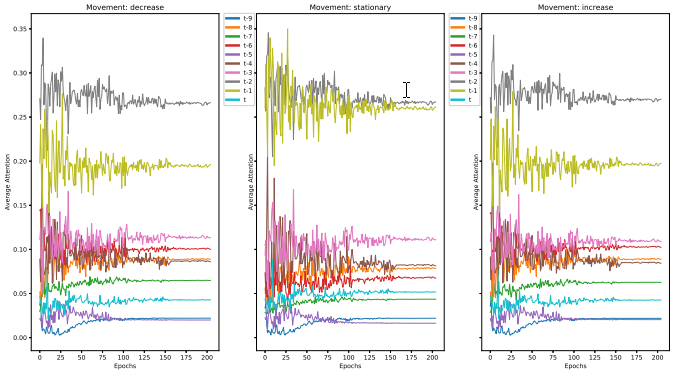
\includegraphics[width=\linewidth]{tseries}
	\end{figure}
	
	\subsection{Limit Order Book}
	A limit order is a type of order to buy or sell a specific number of shares for a set price.
	\begin{definition}[Limit Order Book]
		 A record of outstanding limit orders maintained by the security specialist who works at the exchange. A limit order is a type of order to buy or sell a security at a specific price or better. A buy limit order is an order to buy at a preset price or lower while a sell limit order is an order to sell a security at a pre-specified price or higher.
	\end{definition}
	
	The general purpose is to match buyers and sellers in the market. Most electronic stock exchanges use limit order books in today's market. Generally limit order books are not public information outside of cryptocurrencies. Often, a subscription has to be paid in order to access them. Limit order books contain prices that are "asked" or offered, along with bids which are what people are offering to buy the asset. Each bid and ask has a quantity that tells you how much of the stock is available at the particular price. There is also a tick size set by the exchange which defines the precision of the bid and ask levels. This information can be found more in-depth at \cite{tradientblog.com_2020}. The figure below gives a visual representation of a limit order book.
	
	\begin{figure}[h]
		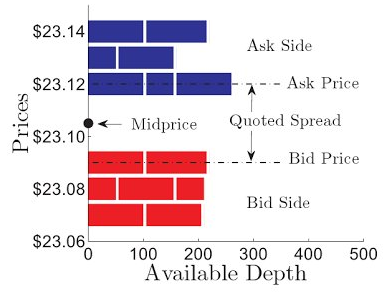
\includegraphics[width=\linewidth]{lobex2}
		\caption{This is depiction of what a limit order book is like. \cite{quantstart}}
	\end{figure}

	These are a good data source to use because they tell the story of how a stock changed throughout the day. These are also considered as a form of time series data.  Thus, many research papers in this field use these as a discussion topic for prediction.
	
	\subsubsection{The Benchmark Dataset}
	The FI-2010 dataset is known as a hallmark benchmark dataset with limit order book data. Most research papers that do tests with limit order books will use this dataset. The data consists of stock data provided by Nasdaq Nordic and comes from Finnish companies Kesko Oyj, Outokumpu Oyj, Sampo, Rautaruukki and Wartsila Oyj. The time period used for collecting that data ranges from the 1st to the 14th June 2010. (This timespan only includes business days that the market is open) The dataset is made up of 10 days for 5 different stocks and 4.5 million total messages. There are 4 metrics for measuring performance while using this dataset. They are mean accuracy, recall, precision, and F1 score.
	
	$$ \text{Accuracy} = \dfrac{TP+TN}{TP+TN+FP+FN} $$
	$$ \text{Precision} = \dfrac{TP}{TP+FP} $$
	$$ \text{Recall} = \dfrac{TP}{TP+FN} $$
	$$ \text{F1} = 2 \times \dfrac{\text{Precision} \times \text{Recall}}{\text{Precision} + \text{Recall}} $$
	
	
	TP and TF represent the true positives and true negatives, respectively,
	of the mid-price prediction label compared with the ground truth, where FP and
	FN represents the false positives and false negatives, respectively. It is noted that the F1 score is the most important of the above equations.  F1 score is based on its ability to only be affected in one direction of skew distributions, in the case of unbalanced classes. It is also the harmonic mean of Precision and Recall.
	  
	  
	This dataset and its properties are described in \cite{benchmarkData}. This paper is often cited for research containing the FI-2010 dataset.
	
	
	\subsection{Bag-Of-Words and Open IE}
	The following comes from \cite{brownlee2017}. The bag-of-words model is a way of representing text data when modeling text with machine learning algorithms. The bag-of-words model is simple to understand and implement and has seen great success in problems such as language modeling and document classification. The source continues with a tutorial on how to create a bag-of-words model.
	
	
	
	For our purposes, the bag-of-words is really good for extracting text information. A vein of stock market analysis incorporates doing event driven correlations with stock price changes. It is often believed that weird drops or rises in the stock market can be explained by some news event that happened. Bag-of-words models are useful to collect this text information for neural networks that aim to predict trends by events that have occurred.
	
	
	A few years later after the bag-of-words idea became prominent, a new idea called Open Information Extraction  (Open IE) emerged. It is the task of generating a structured, machine-readable representation of the information in text, usually in the form of triples or n-ary propositions. It is useful because instead of setting up specific key words that you're looking for like in bag-of-words, you're generating phrases from those words that can actually be useful. This helps piece together clumps of words into events. Let's say they had the words {"Microsoft", "sues", "Barnes", "Noble"}, it can be pieced together as an event that says "Microsoft sues Barnes and Noble". This is much more useful when one is trying to use stock market changes and events to predict what is going to happen.
	
	\section{Pre 2012 Era}
	This section is meant to cover some of the first work accomplished within the field of deep learning and the stock market. There is a large array of papers that have been written with this subject. It is impossible to cover them all, but the goal is to try and cover major works that have happened.
	
	
	In 1965, the question of being able to predict the stock market was starting to get frequently asked. One of the most popular papers ever written on this subject is \cite{behaviorOf}. It is basically a large catalog of many attempts to analyze changes in the stock market. It shows attempts using chaos theory and the Mandelbrot set. It shows articulations to say the stock market is just an independent random walk. The important take away from this article was that it is one of the first analytical works for analyzing the stock market. It is also referenced be many papers that attempt to predict the stock market using deep learning.
	
	
	In 1988, Dr. Halbert White from the University of California, San Diego posted a paper about analyzing IBM Daily Stock Returns in \cite{White1988}. They're trying to analyze stock returns an asset changes using a simple neural network. The study primarily focuses on the one day rate of return for holding the IBM common stock. They created a 3 layer feed forward network modeled after the efficient market hypothesis and the network was aimed to converge on nonlinear least squares using back propagation. They attempted to make the neural network as empirical as possible, however they later declared that this network was not a money machine. They believed that future work would be to make a network based on profit and loss in dollars from generated trades, not squared forecast error like they attempted.
	
	
	In 2001, Blake LeBaron led a study on using an agent based model in order to predict the stock market in \cite{LeBaron2001}. The goal was to create an agent based model that can quantitatively replicate features of financial markets. The goal of simulating the market like the actual stock market was to better understand how the stock market worked. LeBaron noted that analytical models haven't fared well when it came to predicting the stock market, so he aimed to create a toy version of it. Although this research was an initial test, it became a strong foundation for deep learning models in the future.
	
	
	A lot of current research with the stock market and deep learning involves combining the stock market with the news. However, combining deep learning techniques and text analysis for the stock market wasn't really popular until after 2012. In fact, most deep learning and finance work before 2012 was a lot more hit or miss than it is today, with a very large emphasis on the miss. A good showcase of this is presented in [Designing a neural network for forecasting financial and economic time series]. This paper's goal was to provide a practical introduction for designing a neural network to work with economic time series data. It stems to reason that for papers like this one and many others that cite this one have a common issue. When most people are learning about deep learning the time it takes to run a model is always a factor. Deep learning and the stock market was probably ahead of its time until the resources to feasibly process all the data effectively became available. Most research that stems from this paper, and cited by papers later on is work with neural networks trying to handle basic time series data. Stock market research didn't really start hitting strides in the deep learning field until the next section.
	
	\section{2012 to 2017/2018}
	During this era of time the deep learning field has developed a lot more. Convolutional neural networks (CNN), long short term memory networks (LSTM), and other popular deep learning techniques are no longer in the infant stages of being developed. At this time many stock market prediction tools are random forests, auto-regressive moving average models, linear regression models, and other popular basic machine learning techniques. Deep learning research in terms of the stock market started hitting its stride in 2012 and onward. Most of the research that really started happening with stock market prediction was "this model was successful at doing this thing, let's see how it does at predicting stock market changes."
	
	\subsection{S\&P 500 Studies}
	Other notable studies focus on S\&P 500. This is a stock market index that measures the stock performance of 500 companies on the American stock exchange. It covers $80\%$ of the American equity market. While the previous section covered a rough timeline of the FI-2010 dataset research in Finland, this focuses on American market data. S\&P 500 studies don't generally have a set dataset unfortunately like the FI-2010 dataset. These studies generally take a snapshot of a recent time period of several years over the S\&P 500 since all of it's trade data has been accessible to the public. It is common however for the snapshot to be around 1990 to 2015 in recent articles that contain this kind of research. This makes these studies hard to compare or determine what is better, but it is still a significant vein of research in the stock market and deep learning field.
	
	
	\subsubsection{Text Classification Studies}
	This subsection focuses generally on a chain of text classification studies that occurred between 2012 and 2017. These papers are popular among event based stock market prediction community. They brought forth a lot of advancements for the field at the time they were written.
	
	
	There was a study in 2012 that focused on using text classification in order to predict stock returns. It was led by Dr. Luss in \cite{Luss2012}. Text features were extracted from press releases as a bag-of-words. They then value the frequency of these words. They then use multiple kernel learning in order to combine the text features with a support vector machine (SVM) that is valuing movements of financial assets. To increase performance they develop an analytic center cutting plane method. They noted that the text and the SVM by themselves were highly ineffective. However, together they achieved over $55\%$ accuracy with a larger than $\$8000$ profit margin. These results were state of the art at the time.
	
	
	In 2014, a similar study was done in \cite{Ding2014}. In this research, a major thing they did was use events instead of just bag-of-words to help do predictions. This was one of the first papers to use Open IE with stock market prediction. In this research they used a neural network to combine the events and the stock price changes. They were comparing a linear model that they made with this deep neural network. They found the deep neural network to be much more successful, and it had around $60\%$ percent accuracy with a $\$10000$ profit margin. This research was also one of the first to show that event-driven methods with a deep neural network could be an effective form of analyzing the stock market. 
	
	
	A popular study with Deep Learning and stock prediction occurs in \cite{Ding2015DeepLF}. The goal of this project was to use S\&P 500 data to propose a deep learning method for event driven stock prediction. Text features were extracted from press releases as a bag-of-words. In order to learn event embeddings, the researchers use a Neural Tensor Network (NTN). In an NTN, each unit represents values for some combination of attributes rather than for just a single attribute. The NTN works with Open IE to create phrases to help make these events more useful. These events are then fed into a CNN as long-term, mid-term, and short-term events. The convolution layer that holds long-term and mid-term events is followed by a max pooling layer. Short-term events don't go under the covolution operation. To correlate all of these events with stock prices they use a feed forward neural network with one hidden layer. This model got compared against [Using structured events to predict stock price movement: an empirical investigation] and [predicting abnormal returns using text classification]. It ended up being $10\%$ more accurate with index prediction, $5\%$ more accurate with individual stock predictions, and $\$6000$ more profitable than the other models.
	
	\begin{figure}[h]
		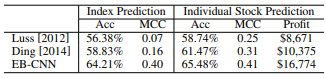
\includegraphics[width=\linewidth]{textSeriesResults}
	\end{figure}
	
	\begin{figure}[h]
		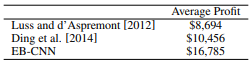
\includegraphics[width=\linewidth]{dollars}
		\caption{For the three papers listed. This is a figure from the third one \cite{Ding2015DeepLF} that compares all three models.}
	\end{figure}
	
	It is interesting to note how the usage of text to help with predictions generally evolved over time with these papers. At first it was just bag-of-words with a basic classifier which became a standard around the world as seen within other papers within this survey and outside of it. Then with Open IE using deep neural networks became much more attractive as the ability to start putting events together became possible. Then, as seen within other fields, enhancing neural networks with extensions made correlating events with stock price changes even easier to catch within the deep neural network models.
	
	\subsubsection{Combining the Private Sector and Education Realm}
	A study in \cite{Krauss2016} had a goal to sort of bridge the gap between the private sector and the educational world when it came to financial research. They train noted that the private sector had these black box tree algorithms and random forests, but were not attempting deep neural networks (DNN). Overall, the random forest outperformed the DNN by a small margin. The researchers noted that careful hyper parameterization optimization could cause the DNN to outperform the random forest, but more research would need to be done. This paper is significant because it showed potential for deep learning and analysis of the S\&P 500.
	
	
	Another study involves research between professors at standard and a Google employee in \cite{Xiong2015}. Starting in 2004, Google has been collecting the daily volume of searches related to various aspects of macroeconomics. This database is available to the public as the Google domestic trends dataset. This research combined 25 different domestic trends with observed S\&P 500 returns and volatility. They split all of this data into a training set that ranges from 2004 to 2012 and a test set that ranges from 2012 to 2015. It is all time series data. To model it they created an RNN that has a single LSTM hidden layer. This model ended up having roughly a $10\%$ improvement on all other models when it came to modeling this volatility. The point of this study was to show potential of deep learning financial time series in the presence of strong noise.
	
	
	Following the previously mentioned studies an attempt at applying an LSTM to \cite{Fischer2017Deep}. They believed that LSTMs are perfect for the S\&P 500 time series data. This is another paper written for the Econstor journal. This article is also aimed at helping bring together the private sector and education realms of research. They found that their basic LSTM model outperfomed the DNN and random forest models. They did note that the LSTM has problems handling a financial crisis. However, it is safe to assume that most machine learning models will have issues with sudden financial crises. We also see from this research paper that LSTMs are worth studying more on this type of financial data to try and see improved results just like earlier in the FI-2010 studies.
	
	\subsection{Notable FI-2010 Studies}
	In 2017 there was a notable CNN model, LSTM model, and a Bilinear Network model that all came out in pretty rapid succession. The CNN paper and the LSTM paper came out at roughly the same time, then the Bilinear Network paper came out after these two and cited them both. They all came from the University of Technology in Tampere Finland, which is the same university that created the FI-2010 dataset.
	
	
	The first of the three is a study led by Dr. Tsantekidis in \cite{Tsantekidis2017F}. They used a CNN that had a 2D convolution layer with 16 filters, a 1D convolution layer with 16 filters and a max pooling layer, 2 1D convolution layers with 32 filters with a max pooling layer following the second one, a fully connected layer with 32 neurons, and a softmax fully connected layer of 3 neurons. This CNN was compared against a support vector machine and a multilayer perceptron model. This paper essentially proved that CNNs are the best approach at that time for modeling this dataset. The F1 score that it achieved was around $60\%$. This was a state of the are score at the time.
	
	
	This next study was also led by Dr. Tsantekidis in \cite{Tsantekidis2017U}. The methodology from this work is based on recurrent neural networks (RNN), that can be used for predicting future mid-price movements from large-scale high-frequency limit order data. They consider the LSTM they come up with to be an improved RNN. They chose the LSTM because it solves the problem of vanishing gradients, which is virtually impossible for an RNN to learn to correlate temporally distant events. This is achieved by protecting its hidden activation using gates between each of its transaction points with the rest of its layers. The hidden activation that is protected is called the cell state. The input is a sequence of vectors that represent the LOB depth at each time step. It should be noted that the error isn't propagated until after the first 100 recurrent steps, which the authors call the "burn-in" sequence. They also noted that the LSTM would overfit the data if more than 64 hidden neurons were used. Overall, the LSTM acheived an F1 score of around $62\%$ which is a supposedly a little better than the CNN in the previously mentioned paper.
	
	
	Not long after the previous paper a different study was done using a bilinear network in \cite{Tran2017}. This study was meant to take an approach at approximating the dataset with a much shallower model. It uses a Temporal Attention augmented Bilinear Layer (TABL). It has three different configurations known as A, B, and C. The input is a matrix that is $40 \times 10$ which contains prices and volumes of the top 10 orders from bid and ask side ($40$ values) spanning over a history of $100$ events. All three configurations end with a $3 \times 1$ bilinear softmax layer. Configurations B and C have a $120 \times 5$ bilinear relu layer. Configuration C has a $60 \times 10$ bilinear relu layer before the previously described layer. Of the three configurations, C seems to be the one that consistently performs the best. Configurations B and C also consistently outperformed the CNN and LSTM models listed above.
	
	
	There were several studies that followed the previous ones, except this one scored remarkably well on the FI-2010 dataset. This study is covered in \cite{deepLOB}. They use standard convolutional layers, a LSTM layer, and an Inception Module which is used to allow more efficient computation in deep networks with dimensionality reduction. The inception module was meant to do feature extraction as the data from the limit books are extremely noisy. This is one of the first attempts to use an inception module on this kind of problem within the field. The tests they did blew all of the standard models out of the water. It seems that this model was the one of the first to achieve above $80\%$ accuracy on the dataset. According to this study the best F1 score at the time was around $78\%$ which was achieved by [Temporal Attention Augmented Bilinear Network for Financial Time-Series Data Analysis] after these authors reran that model. It is hard to officially determine which of the two methods is better. The figure below depicts a table that is used in the studies that were just discussed in the previous papers. 
	
	\begin{figure}[h]
		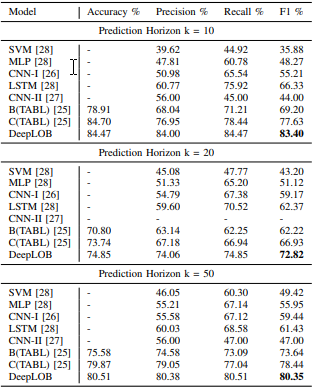
\includegraphics[width=\linewidth]{fi2010}
		\caption{This is the data table that the previous papers would use to compare the models. This one came from \cite{deepLOB}. The Prediction Horizon k = "some number" stands for the amount of k-folds cross validation that were done.}
	\end{figure}
	
	
	In 2018, a group of researchers decided to look into temporal bag-of-features with this dataset in \cite{Passalis2018}. This research aims to extract features from the limit order book data in order to do the predictions. Although this idea seemed good, bag-of-features doesn't work well with limit order book data. The best F1 score this research achieved was around $50\%$. It can be found that this is a common theme with research in this field where external tricks that have improved performance in some areas doesn't in this one.
	
	\section{General Notable Studies 2017 Onward}
	Most of the notable studies that capitalize on previously mentioned work don't fall under a general umbrella. It seems that an explosion happened within the field in 2017. Most explosions in the deep learning field seemed to have happened a couple years ago, but it seems that most ground breaking stock market research with deep learning only started happening recently. This section aims to capture a variety of work for when deep learning really started gaining it's foothold in the stock market prediction realm. 
	
	
	 In mid 2017 a study was posted that tried applying CNNs to High-Frequency Markets in \cite{Doering2017}. This study used limit order book data as well as order-flow information to conduct its study. The CNN was able to achieve $50\%$ accuracy at predicting trends and around $68\%$ at predicting the volatility. For being in a high frequency market these results are pretty groundbreaking. However, a major drawback is that the time period the data covered was only 217 days. This is an incredibly short time period. The author noted that the network felt rather black boxy with decisions that it was making. To contrast this study against many other studies, the time period is usually several years worth of data. This is an example of a study that went really well, but it is hard to tell how much empirical value it actually offers to the field.
	 
	 
	 A seperate study in 2017 that hasn't been covered yet includes hybrid neural networks attempting to learn time series trends in \cite{Lin2017}. They created a network that they named as TreNet. TreNet contains a CNN, LSTM, and predictive functions. It learns a joint feature used for trend prediction. They evaluated TreNet on power consumption, gas sensor, and stock exchange data. The stock exchange data included NYSE stocks from 1950 to 2016. TreNet was then compared against many baseline models such as a standard CNN, LSTM, SVM, and several other models. Overall TreNet had the lowest RMSE score of all the models. Given how successful other models have been up until this one, it is almost safe to assume that a hybrid model would be moderately successful at analyzing stock trends. This article proves this to be the case.
	 
	 At the end of 2017 another follow up to the previously mentioned studies that gained some traction occurred. This study in \cite{Zhou2018StockMP} was led by Dr. Zhou in China. They propose a generic framework employing Long Short-Term Memory (LSTM) and
	 convolutional neural network (CNN) for adversarial training to forecast high-frequency stock market. By this point LSTMs were starting to become the new normal in the world of stock market prediction due to how well they naturally handle the noisy time series data. In this research the LSTM was used as a generative model. It is combined with discriminative model is based on the CNN architecture and performs convolution operations on the one-dimensional input sequence. It's job was to say whether the input was part of the generative model or whether it came from the Chinese stock market. This is one of the first research papers that took an adversarial approach so as to mimic an good experienced stock trader making stock predictions. They applied this idea to the year 2016 in the Chinese stock market. This network was meant to try and mimic time periods when traders prefer high volatility stocks, and times when they prefer low volatility stocks. This paper also employed root mean squared relative error (RMSRE) for testing their model. They believed that this method helped produce a uniform comparison of the results for 42 stocks. Their model ended up being better than all baseline methods at the time. 
	 
	 
	 Another notable study that used S\&P 500 data is \cite{Chong2017}. This paper proposed a deep feature learning-based stock market prediction model. The aim of this research was to do a comprehensive study of applying deep neural networks to the stock market. The paper concluded that the deep learning field is constantly growing, thus their research here could be invalidated at any moment. It should be noted that this paper came out at around a similar time frame the LSTM model came out in the previous section. This study is worth mentioning because it tried to empirically study all the work that had happened within the deep learning field up until what seems to be the beginning of 2017. Most of the major strides within the field that have happened occurred mid 2017 and after.
	 
	 
	 It should often be noted that even though some of these models have been moderately successful at predicting stock accuracy, the value of a human expert can go a long way. In Germany Dr. Kraus lead a study that seeks to improve the machine learning business interaction in \cite{Kraus2017}. For data they have a corpus that contains over 13000 words of regulated German announcements. They ignored any news that dealt with penny stocks, which falls in line with the idea of only analyzing the S\&P 500 or the FI-2010 data from previously discussed papers. This model uses transfer learning to combine the corpus data with current financial and new data in a deep learning model that consists of an RNN and a LSTM. This idea outperformed all the baseline models at the time which were non-deep learning models. The paper noted that this model was better able to assist experienced traders with their decisions. 
	 
	
	 The reason the previous paper is important is because it is another case of somebody applying deep learning models that include a LSTM and having greater success predicting stock market trends than the standard non-deep learning models. This paper has been able to showcase moderate success of deep learning within the American, Finnish, German, and Chinese stock markets. LSTMs aren't necessarily the answer to what should be used to predict stock market changes, however it is worth noting that in pretty much any research paper that has been published in 2017, they outperform the standards.
	 
	 
	 In the financial world, one of the most well known forecasting methods for market analysis is the auto-regressive moving average (ARMA). An enhanced version of this is auto-regressive integrated moving average. For external knowledge on forecasting ARIMA models check out \cite{prahakaran_2019}. We've also found that LSTMs are very good at predicting stock market trends compared to most baseline models. A team at Texas Tech sought to do an empirical comparisons of LSTMs and ARIMA models in \cite{Namini2018}. This study compared the two methodologies in terms of trying to minimize the error rates in prediction as much as possible. They used time series data that ranged from January 1985 to August 2018 off of the Yahoo Finance website, and it covered a wide range of different stocks. They articulated their ARIMA and LSTM implementations so that they are easy to replicate. The study uncovered that LSTMs are significantly better than ARIMA models by a large margin. This shows that deep learning concepts need to be used more in the stock market/forecasting world as a whole. LSTM implementations are finding continued success.
	 
	 
	 Another research study that compared ARIMA models vs common deep learning models in \cite{Hiransha2018}. The main difference between this paper and the previous paper that was just discussed is the markets and amount of models that were compared. This paper compared an MLP, RNN, LSTM, and CNN vs the ARIMA model with stocks from NSE and the NYSE. These are two of the largest stock markets in the world and they are different then previously discussed markets in this paper. It was then found that the ability for the deep learning models to find underlying dynamics within the market made them perform significantly better. This paper said that it would be interesting to see how hybrid models perform at stock market prediction.
	 
	 
	 This next paper attempts to design an RNN to predict the stock market in India for \cite{Sachdeva2019}. They used historical data of INFOSYS Ltd from NSE IT sector and NSE NIFTY 50 from Yahoo finance. They ended up using an LSTM model because it helped them with the vanishing gradient descent problem that they ran into. forecast stock prices of INFOSYS LTD. and M\&M from NSE Indian stock exchange and also for predicting the NIFTY50 index. The best accuracy obtained for Infosys Ltd. dataset using 60 time steps and RMSprop as the optimizer was $97.64\%$. From the results obtained, it is clear evident that the deep learning models are capable of forecasting the NSE stock market. It is yet another example of an LSTM having great success predicting stock prices.
	 
	 
	 One topic that hasn't been talked about yet in this survey is reinforcement learning. Reinforcement learning appears to be a rather under explored technique in terms of stock trading. Dr. Quang-Vinh Dang in Vietnam did research in 2019 in \cite{Vinh2019}. They study a Deep Q-Network (DQN) for stock trading. The goal is not only to have good stock prediction, but to also use reinforcement learning to be able to tell when to buy and sell stocks. They employed a simple greedy strategy that bought when they thought the stock would go up, and sold when they thought the stock would go down. They visualize the performance of four models vanilla DQN, double DQN, dueling DQN, and a baseline LSTM model on the Google stock. The dueling DQN seemed to be the most stable of the networks, however the standard DQN was the most profitable. The downside to the DQN is that it was also the most volatile of the networks. This made sense because of its basic greedy approach algorithm that was explained a little earlier. It stands to reason that no professional would want to use these networks yet to do stock prediction. However, over time with more innovation and teaching the network better stock management strategies it could stand a chance. Perhaps in the future this approach will surpass LSTMs in general. The peak performance of the DQN surpassed the LSTM so, the goal is to make that performance more consistent.
	 
	 
	 It is rather interesting that reinforcement learning is one of the most underutilized techniques when it comes to stock trading. This could be because of several reasons. The first reason being that it is farther behind all other techniques in terms of research and has really only been applied to video games, mapping problems, and other similar challenges. Stock trading has also been a research issue in the professional side of research than the educational side. It'll be interesting to see how this topic and the stock market advances over the next few years.
	 
	 
	 A rather recent study that occurred in 2020 aims to predict the stock market using a deep convolutional LSTM (Deep-ConvLSTM) in \cite{Kelotra2020}. The major innovation that comes from this article is the preprocessing of all the data that happens in the model. They take in all the information possible about a stock within the day from the opening price to the closing price. They then use feature extraction of technical indicators as part of their feature clustering process, and the other part involves a sparse-fcm algorithm. They then feed that and Rider-based monarch butterfly optimization into their Deep-ConvLSTM. A figure from their article is listed below to present a picture of what the research is doing.
	 
	 \begin{figure}[h]
		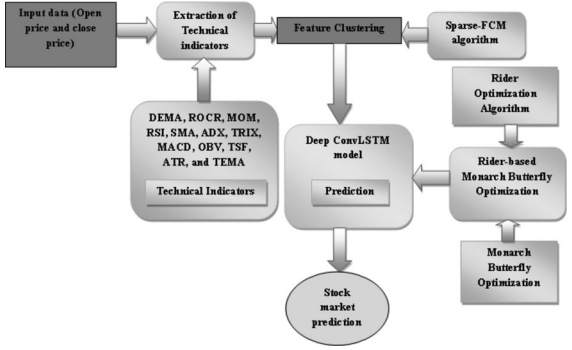
\includegraphics[width=\linewidth]{butterfly}
		\caption{For more information on how this model works please check out \cite{Kelotra2020}}
	 \end{figure}
	 
	 
	 The experimentation of the proposed method is carried out by using the metrics, such as MSE and RMSE, in the presence of the data collected from six live stock markets. The proposed method produces the minimum MSE of 7.2487 and RMSE of 2.6923. There is a high chance this is the new "state of the art" model even though it hasn't been around for even half a year yet at the time this paper was written. It has successfully taken feature extraction and stock market data to a whole new level. Earlier on in the paper it was mentioned that the technology didn't really exist for complex models to analyze the large noisy chaotic nature of the stock market. With the advent of a model like this one and others that were talked about before it, the technology to do crazy experiments like this one is more than available.    
	 
	\section{Overall Remarks}
	Unfortunately, one topic that goes a little unnoticed with this topic is calibration. It should be noted that there were studies with financial calibration in [\cite{Itkin2019}, \cite{Culkin2017}, \cite{Hirsa2019}]. Option pricing is typically the route that researchers take when doing calibration research on models within the financial field. This research however is generally out of the scope of this paper, but would be interesting to analyze in the future.

	
	One overall discussion to have is the type of stocks that were being evaluated in most of these papers. Most stock research is on mid-price level stocks. It is hard not to notice that not much research occurs at the high price stock range. Things to note about that is when price fluctuations. When a large price stock change it is by a large or small amount. However, when talking about large and small it is very relative. Say that the stock that is being talked about is Google which is currently at $\$1276.60$ at the time this paper is being written. Most stock prices are much smaller. A shift by $\$50$ is "normal" for a Google stock. A price fluctuation of that much for a mid price stock means something drastically major has happened. Since most of the market is mid price, these deep learning models are going to have/had major problems predicting price fluctuations for large price stocks. Thus, it is hard to find research on stocks at such a high price. Mid price stocks make up a vast majority of the market, thus most of the deep learning and finance community has done their research on those kind of stocks. 
	
	
	Throughout this paper it has been shown that deep learning and the stock market share a deeper connection than has been previously discovered so far. We can only be optimistic that feature extraction of these stocks and the way these methods perform will only improve our understanding of being able to predict the stock market. What seemed like an impossible challenge several years ago, is now just a really challenging problem to solve. Improvement will probably happen at a much slower rate now then it did between the 2012 and 2020 window, but we can only be optimistic that the stock markets around the world stay in the chaotic state that it has always been in.
	
	\section{Conclusion}
	The future of deep learning and the stock market is as cloudy as its past is. The stock market is a game full of risks. Unforeseen events like the coronavirus are hard to predict. It is still unknown if a deep neural network of any kind can cope with drastic events that last for unknown periods. 
	
	
	The standards before deep learning were not that great, so that isn't saying much. These methods do bring qualitative science as a whole one step closer to understanding the inner workings of the stock market from a theoretical perspective.
	
	\Urlmuskip=0mu plus 1mu \relax
	% bib-style provided for ICML 2018
	\bibliographystyle{icml2018}
	
	% the bibliography command should contain the name of your .bib file, minus the
	% extension.
	\bibliography{templateBibliography}
	
	
\end{document}